\documentclass{beamer}
\mode<presentation>
{
  \usetheme{Darmstadt}
  \definecolor{BYUBlue}{RGB}{00,22,55}
  \definecolor{BYUTan}{RGB}{232,211,175}
  \usecolortheme[named=BYUBlue]{structure}
  \setbeamercolor*{palette primary}{use=structure,fg=BYUBlue,bg=lightgray}
  \setbeamercolor*{palette quaternary}{fg=white,bg=lightgray!0!BYUBlue}
  \setbeamercolor{frametitle}{fg=BYUBlue,bg=BYUBlue!10}
  \setbeamertemplate{items}[circle]
  \setbeamertemplate{blocks}[rounded][shadow=True]
  \setbeamertemplate{navigations symbols}{circle}
}

\usepackage{graphics}
\usepackage[english]{babel}
\usepackage[utf8]{inputenc}
\usepackage{times}
\usepackage{forest}
\usepackage{subfigure}
\usepackage{caption}
\captionsetup{labelformat=empty}% redefines the caption setup of the figures environment in the beamer class.
\usepackage[T1]{fontenc}
\usepackage{array}
\usepackage{amsmath,amssymb}
\usepackage{booktabs}
\usepackage{colortbl}
\usepackage{array}
\usepackage{threeparttable}
\usepackage{multirow}
\usepackage{amsthm}
\usepackage{float,graphicx,color}
\usepackage{graphics}
\usepackage{multicol}
\usepackage{natbib}
\usepackage{color}
\usepackage{hyperref}
\hypersetup{colorlinks, urlcolor=blue}
\usepackage{threeparttable}
% \usepackage[format=hang,font=normalsize,labelfont=bf]{caption}
% \usepackage{subcaption}
\usepackage{delarray}
\usepackage{amssymb}
\usepackage{setspace}
\usepackage{placeins}
\usepackage{multirow}
\usepackage{mathtools}
\usepackage{animate}
\usepackage{bm}
\usepackage{amsmath,bm}
\usepackage{amssymb}
\usepackage{amsthm}
\newtheorem*{thm}{Theorem}
\theoremstyle{definition}
\newtheorem*{defn}{Definition}
\newcommand\ve{\varepsilon}
\newcommand\norm[1]{\left\lVert#1\right\rVert}
\DeclareMathOperator*{\argmin}{argmin}

% Python code blocks --------------------------------------
\usepackage{pythonhighlight}
\usepackage{tcolorbox}
\definecolor{codegreen}{rgb}{0,0.6,0}
\definecolor{codegray}{rgb}{0.5,0.5,0.5}
\definecolor{codepurple}{rgb}{0.58,0,0.82}
\definecolor{backcolour}{rgb}{0.95,0.95,0.92}

\lstdefinestyle{mystyle}{
    backgroundcolor=\color{backcolour},
    commentstyle=\color{codegreen},
    keywordstyle=\color{magenta},
    numberstyle=\tiny\color{codegray},
    stringstyle=\color{codepurple},
    basicstyle=\ttfamily\footnotesize,
    breakatwhitespace=false,
    breaklines=true,
    captionpos=b,
    keepspaces=true,
    numbers=left,
    numbersep=5pt,
    showspaces=false,
    showstringspaces=false,
    showtabs=false,
    tabsize=2
}

\lstset{style=mystyle}


\title[OG-Core Examples: Prod-Mort-TFP]{OG-Core Examples: \\ TFP, Productivity, Mortality Shocks}

\author[DeBacker and Evans]{\textbf{Jason DeBacker} \inst{1} \and \textbf{Richard W. Evans} \inst{2}}
\institute[shortinst]{\inst{1} University of South Carolina, Department of Economics \and
\inst{2} Abundance Institute, Open Research Group, Inc.}

\date[Short Occasion]{\textbf{January 15, 2026} \\ United Nations, Philippines}

\begin{document}

\begin{frame}
  \titlepage
\end{frame}


\section{Intro}

  \begin{frame}
    \frametitle{Examples}
    \begin{itemize}
      \item Tax Cuts and Jobs Act (TCJA) Dynamic Analysis
      \vspace{5mm}
      \item Revenue and Macroeconomic Effects of a 70\% Marginal Tax Rate
      \vspace{5mm}
      \item A Detailed Macroeconomic Analysis of President Biden's 2020 Campaign Tax Proposals
      \vspace{5mm}
      \item The Macroeconomics of Improving Biological Aging
    \end{itemize}
  \end{frame}


\section{TCJA}

  \begin{frame}
  \frametitle{TCJA Dynamic Analysis}
    \begin{block}{}
      DeBacker, Jason and Richard W. Evans, ``\href{http://www.openrg.com/dynamic-analysis-of-tax-cuts-and-jobs-act/}{Dynamic Analysis of Tax Cuts and Jobs Act},'' \textit{Quantitative Notes}, 2018-1, (February 2, 2018).
    \end{block}
    \begin{itemize}
      \item GDP growth in first 8 years (1-2\% increase)
      \item Significant crowding out as debt increases
    \end{itemize}
  \end{frame}

  \begin{frame}
  \frametitle{TCJA Macro variables, closed economy}
    \begin{figure}[htb]\centering
    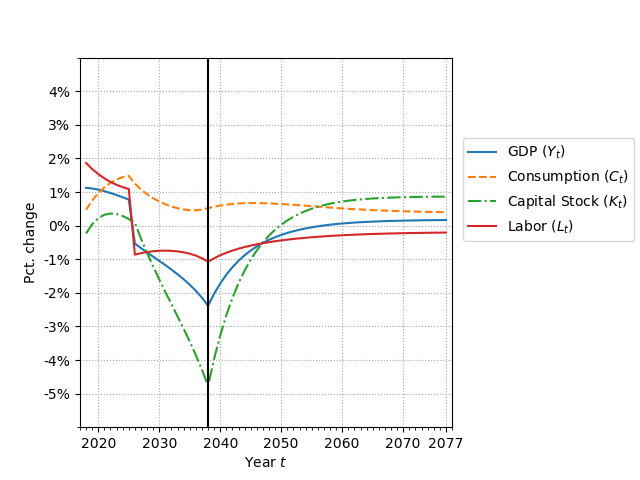
\includegraphics[scale=0.6]{./images/YCIKL_dif_flex_closed.png}
    \end{figure}
  \end{frame}

  \begin{frame}
  \frametitle{TCJA Fiscal variables, closed economy}
    \begin{figure}[htb]\centering
    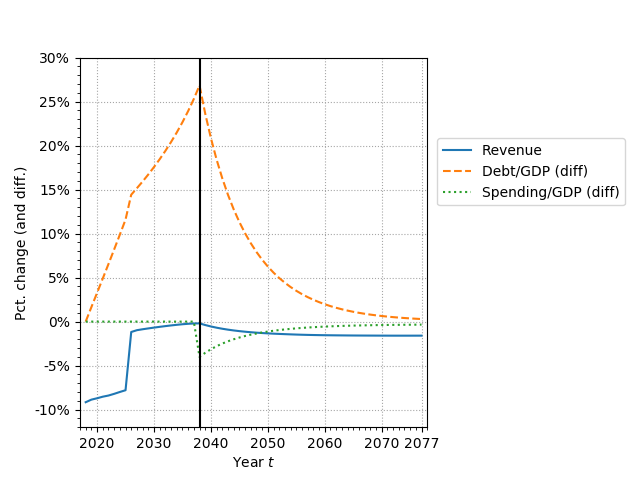
\includegraphics[scale=0.6]{./images/RevDYGY_dif_flex_closed.png}
    \end{figure}
  \end{frame}


\section{Biden 70\%}

  \begin{frame}
  \frametitle{TCJA Dynamic Analysis}
    \begin{block}{}
      DeBacker, Jason and Anderson Frailey, ``\href{http://www.openrg.com/revenue-and-macroeconomic-effects-of-70-marginal-tax-rate/}{Revenue and Macroeconomic Effects of a 70\% Marginal Tax Rate},'' \textit{Quantitative Notes}, 2019-1, (March 4, 2019).
    \end{block}
    \begin{itemize}
      \item Can raise between \$5B and \$250B per year
      \item Reduce GDP in short run between 0.1\% and 1.7\%
    \end{itemize}
  \end{frame}

  \begin{frame}
  \frametitle{70 Percent Federal Revenues Change}
    \begin{figure}[htb]\centering
    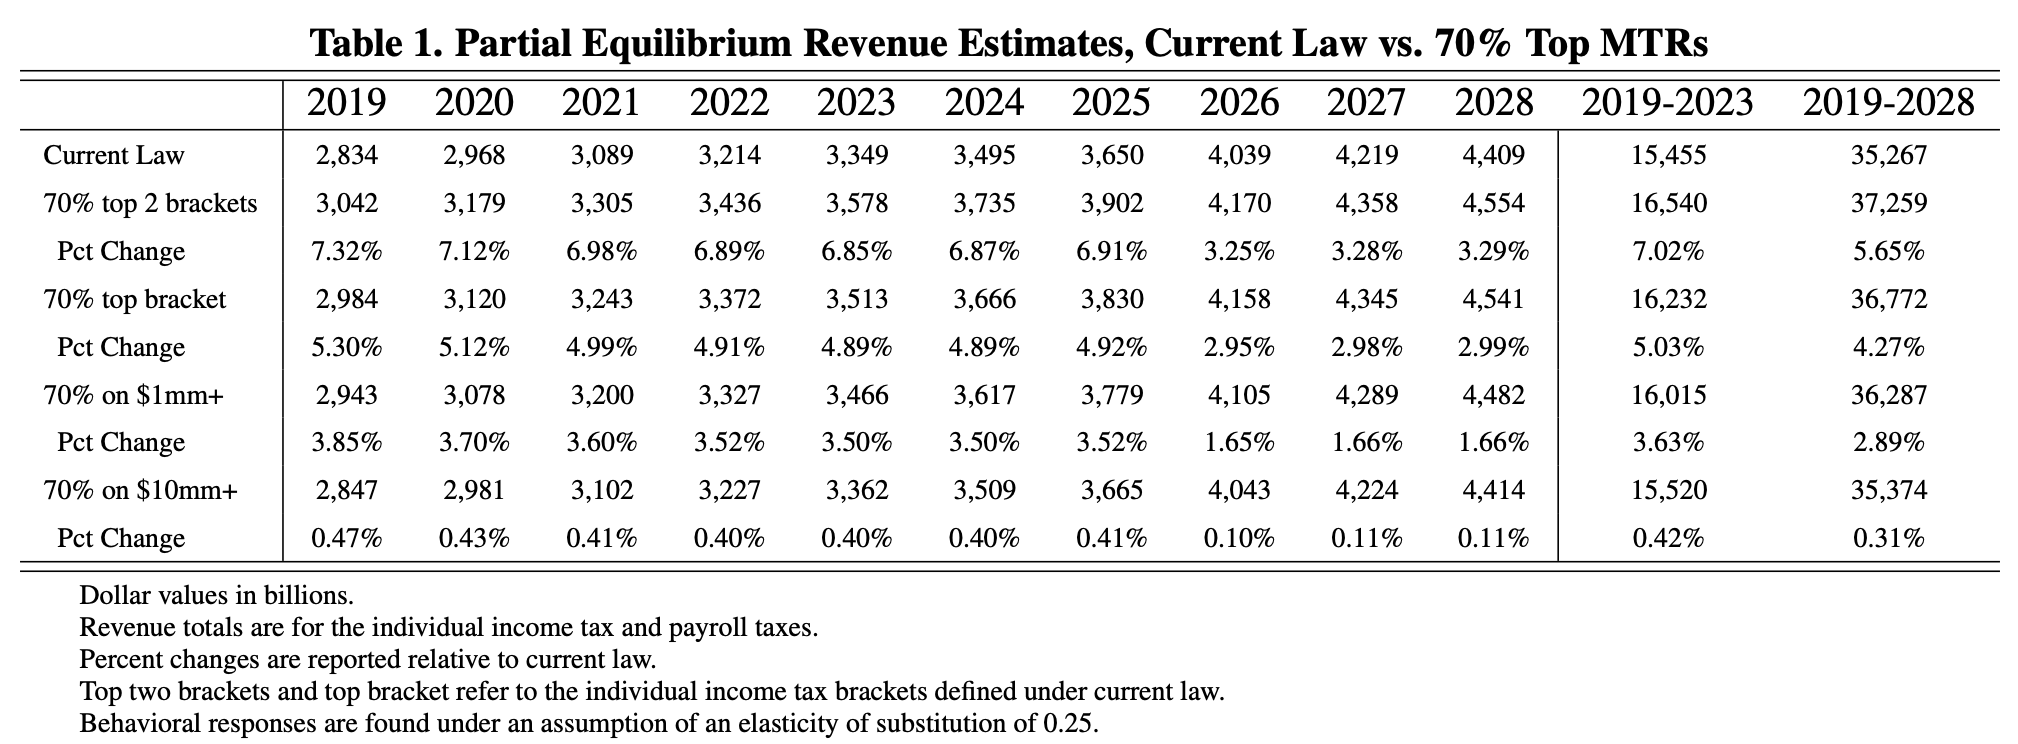
\includegraphics[scale=0.33]{./images/70pctTbl.png}
    \end{figure}
  \end{frame}

  \begin{frame}
  \frametitle{70 Percent Incidence}
    \begin{figure}[htb]\centering
    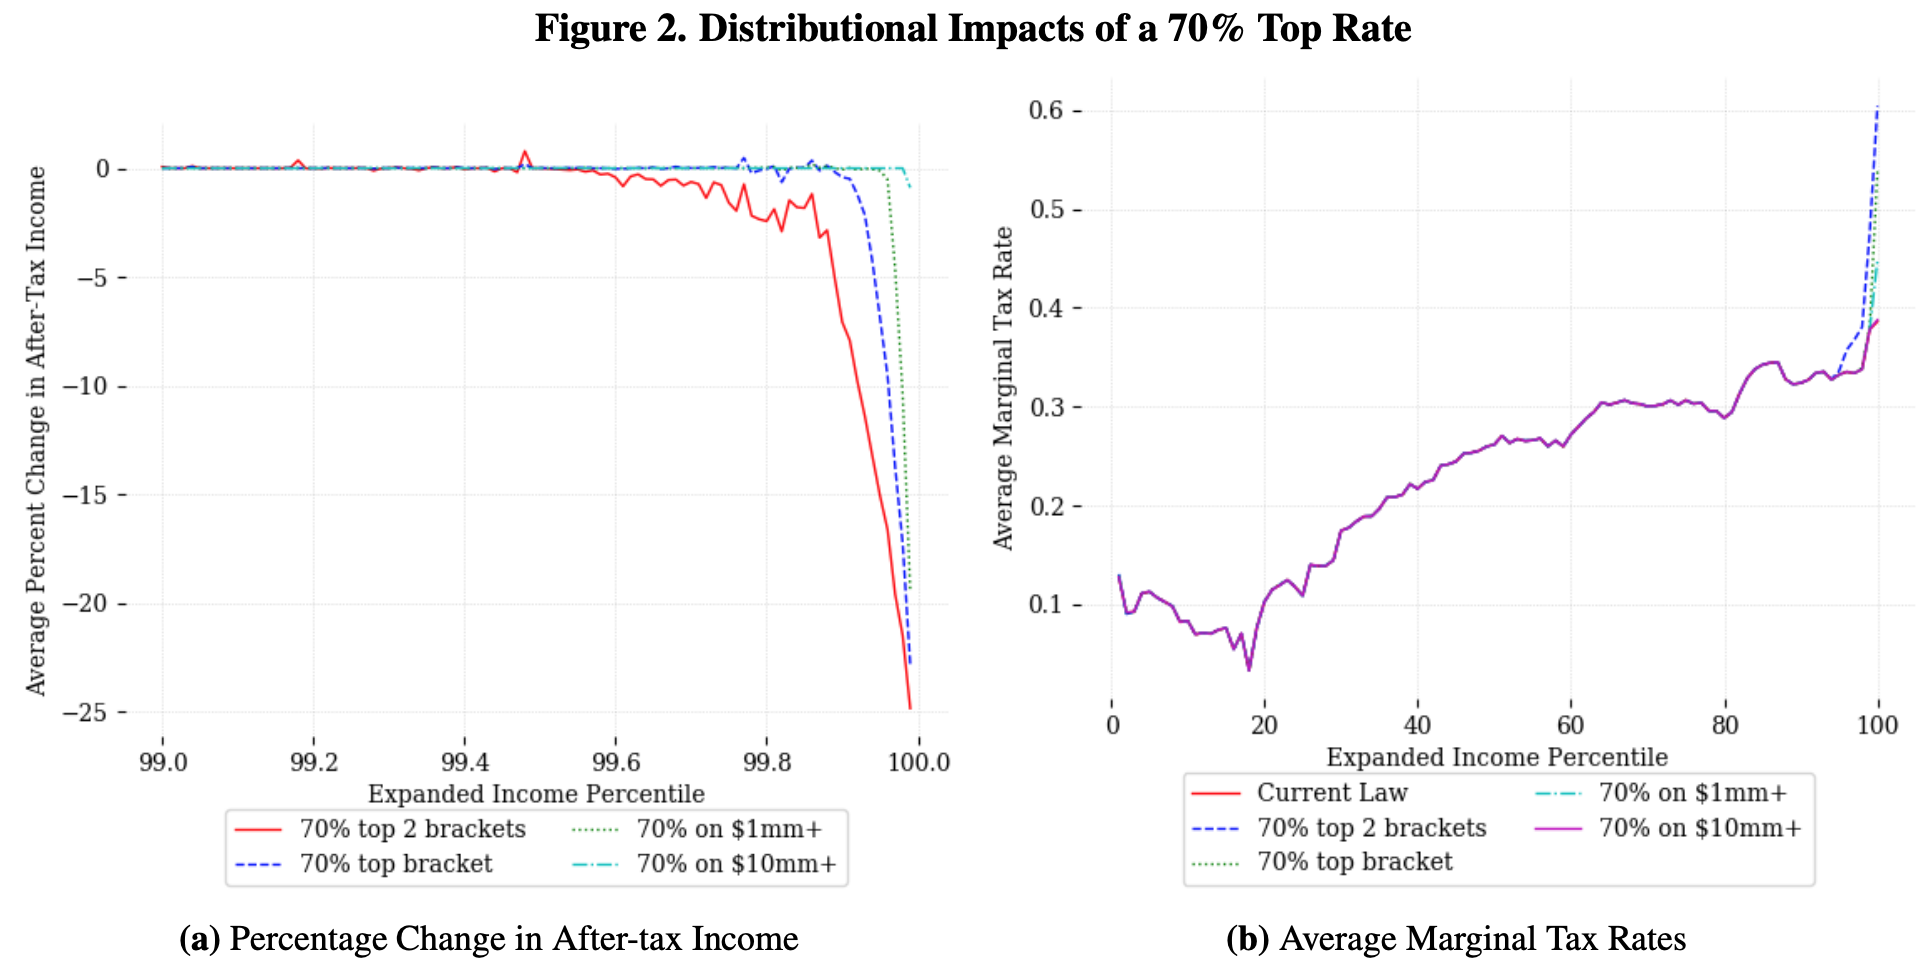
\includegraphics[scale=0.33]{./images/70pctFig.png}
    \end{figure}
  \end{frame}

  \begin{frame}
  \frametitle{70 Percent GDP change}
    \begin{figure}[htb]\centering
    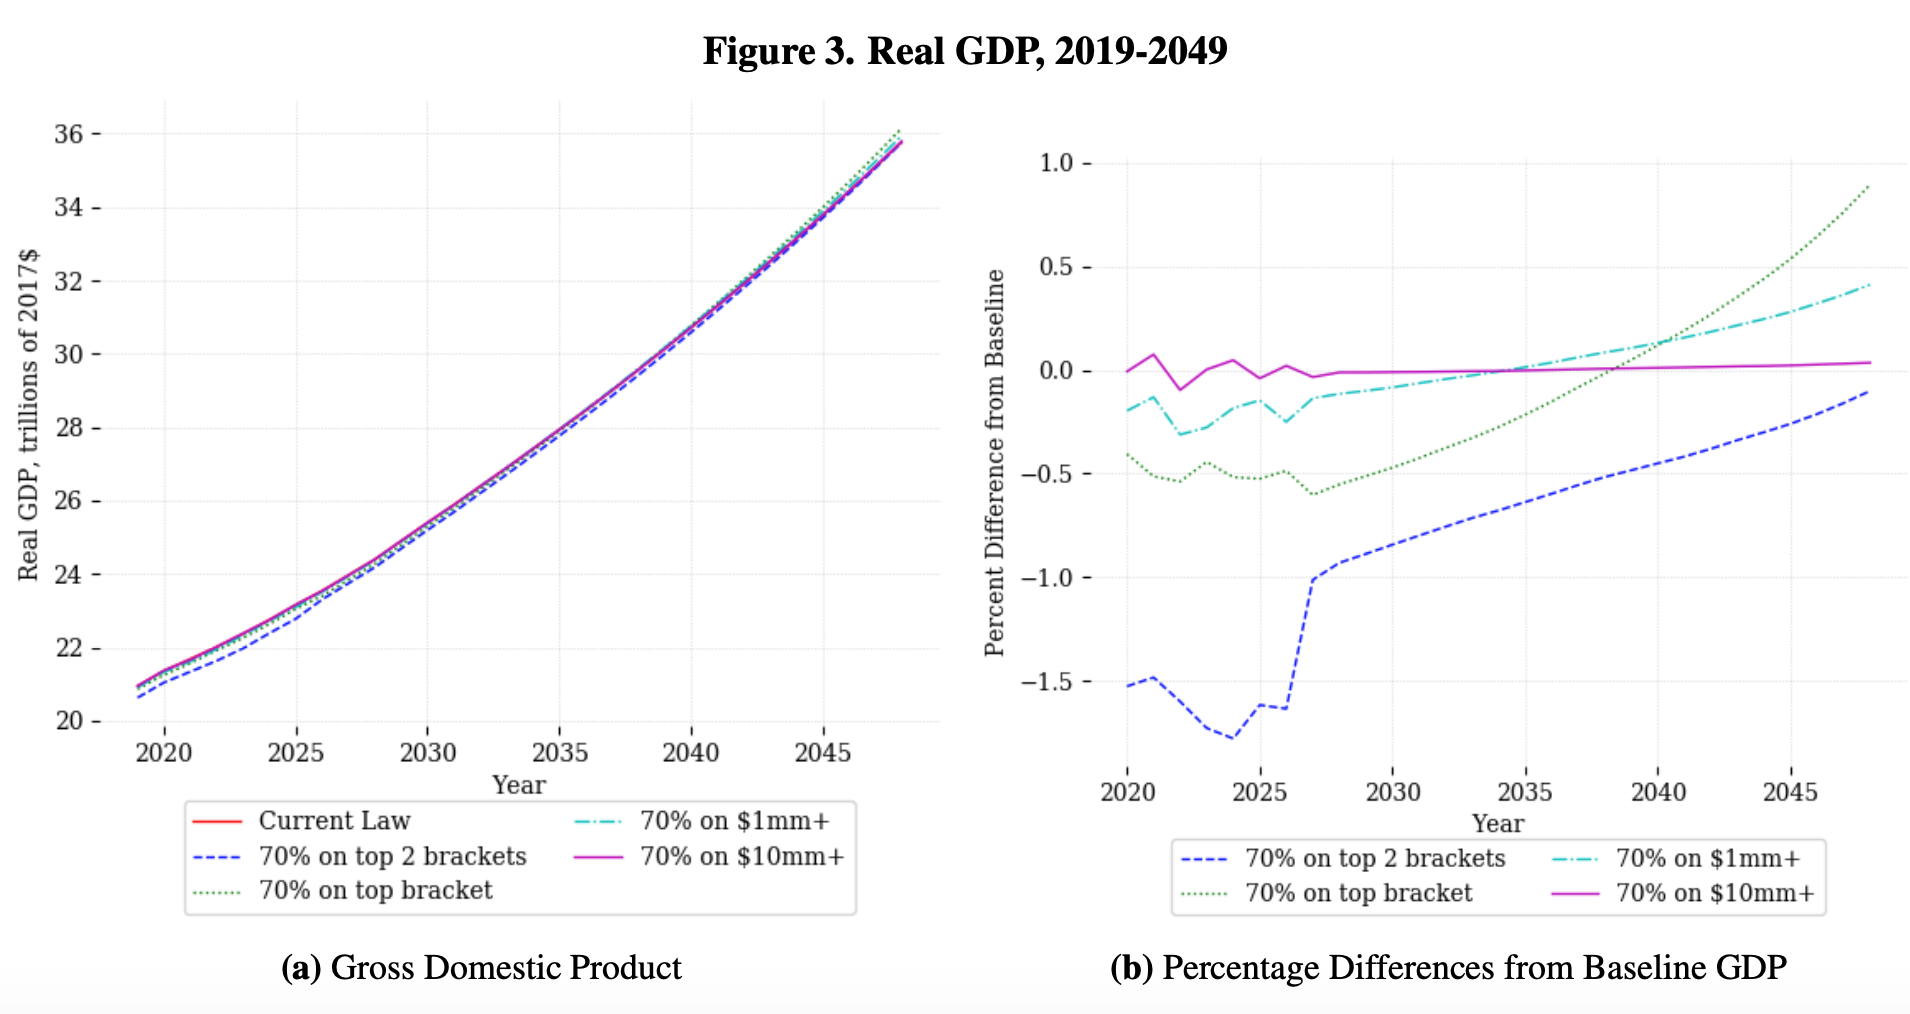
\includegraphics[scale=0.3]{./images/70pctGDP.png}
    \end{figure}
  \end{frame}

\section{Biden 2020}

  \begin{frame}
  \frametitle{Analysis of President Biden's Campaign Proposals}
    \begin{block}{}
      DeBacker, Jason, Richard Evans, and Benjamin Page, ``\href{https://www.taxpolicycenter.org/sites/default/files/publication/162562/a-detailed-macroeconomic-analysis-of-president-bidens-2020-campaign-tax-proposals_1.pdf}{A Detailed Macroeconomic Analysis of President Biden's 2020 Campaign Tax Proposals},'' \textit{Tax Policy Center Working Paper}, July, 2021.
    \end{block}
    \begin{itemize}
      \item Debt reduction crowds in private capital in medium term
      \item We provide a sensitivity analysis to various parameter values
    \end{itemize}
  \end{frame}

  \begin{frame}
  \frametitle{Biden Dynamic Analysis}
    \begin{figure}[htb]\centering
    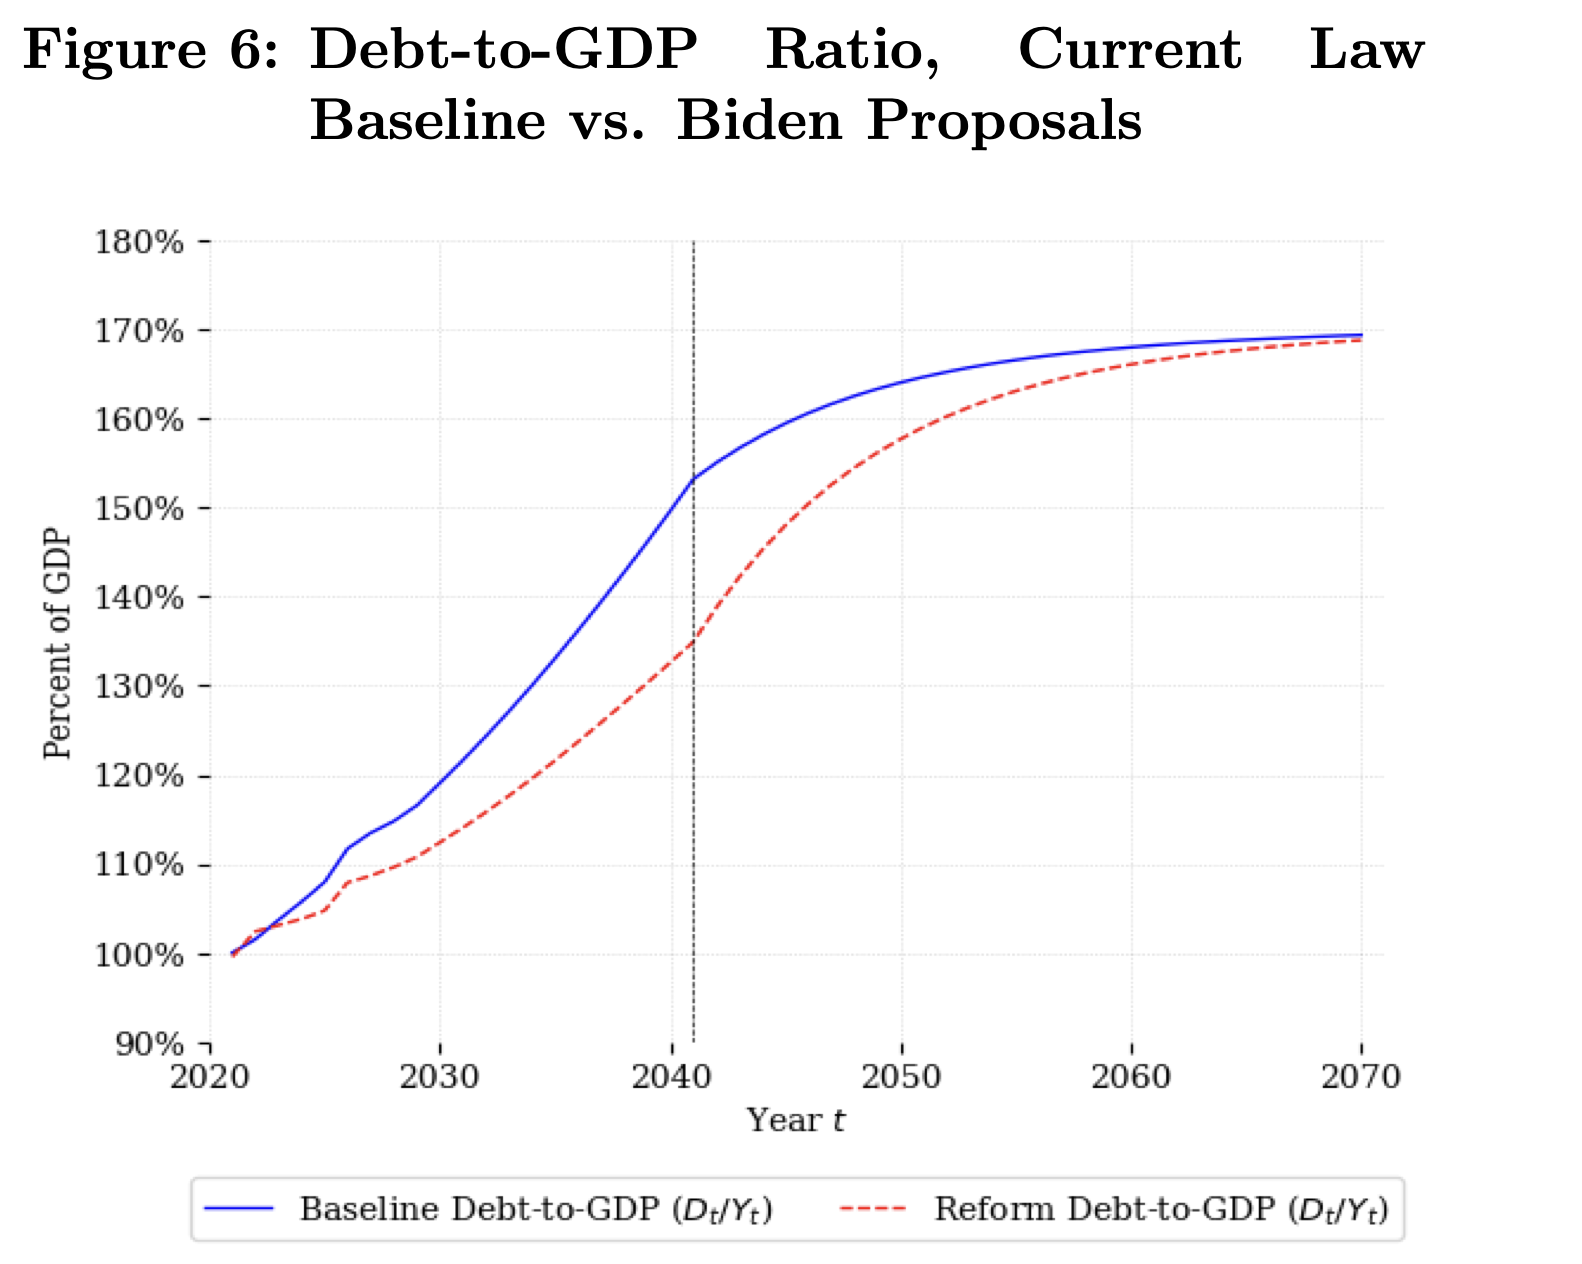
\includegraphics[scale=0.32]{./images/BidenFig6a.png}
    \end{figure}
  \end{frame}

  \begin{frame}
  \frametitle{Biden Dynamic Analysis}
    \begin{figure}[htb]\centering
    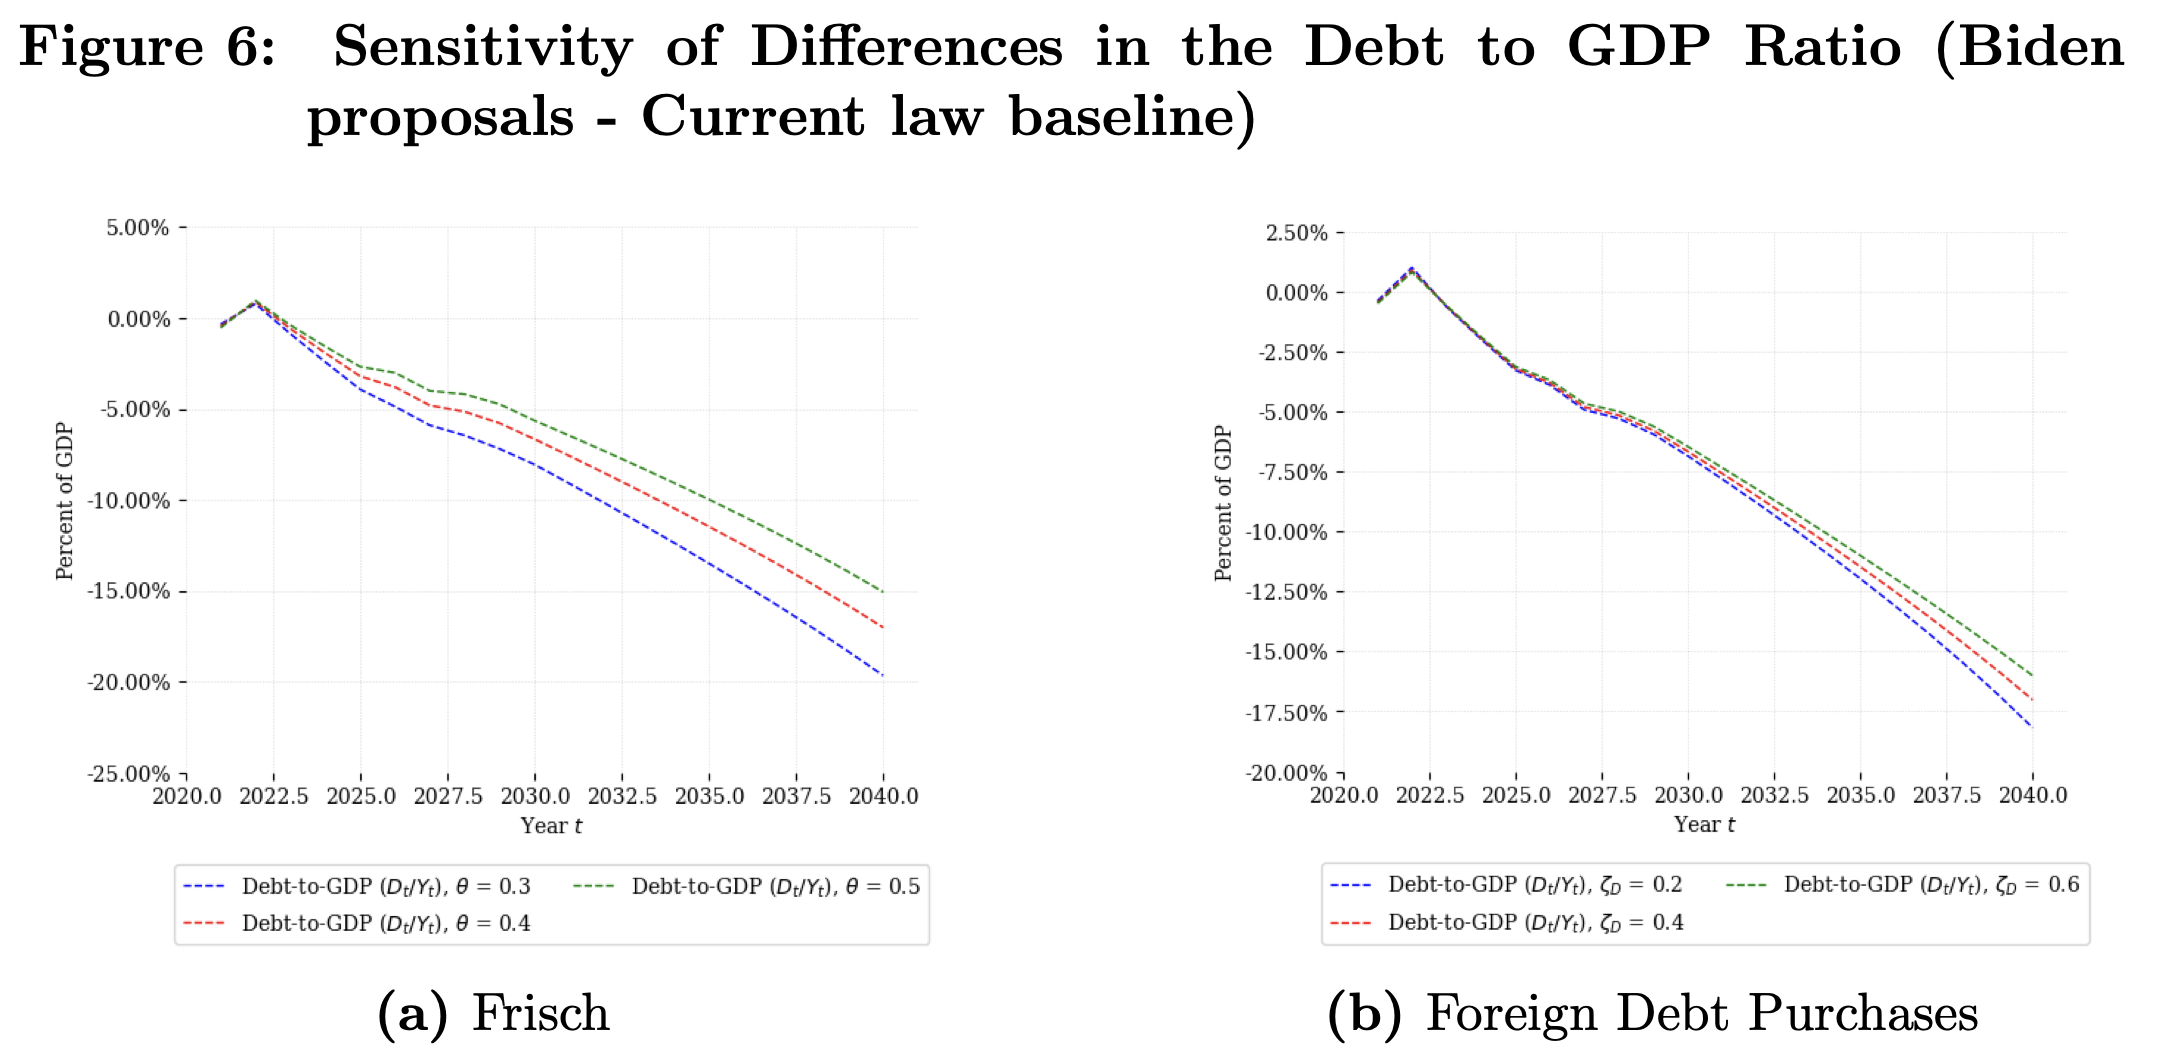
\includegraphics[scale=0.27]{./images/BidenFig6.png}
    \end{figure}
  \end{frame}

  \begin{frame}
  \frametitle{Biden Dynamic Analysis}
    \begin{figure}[htb]\centering
    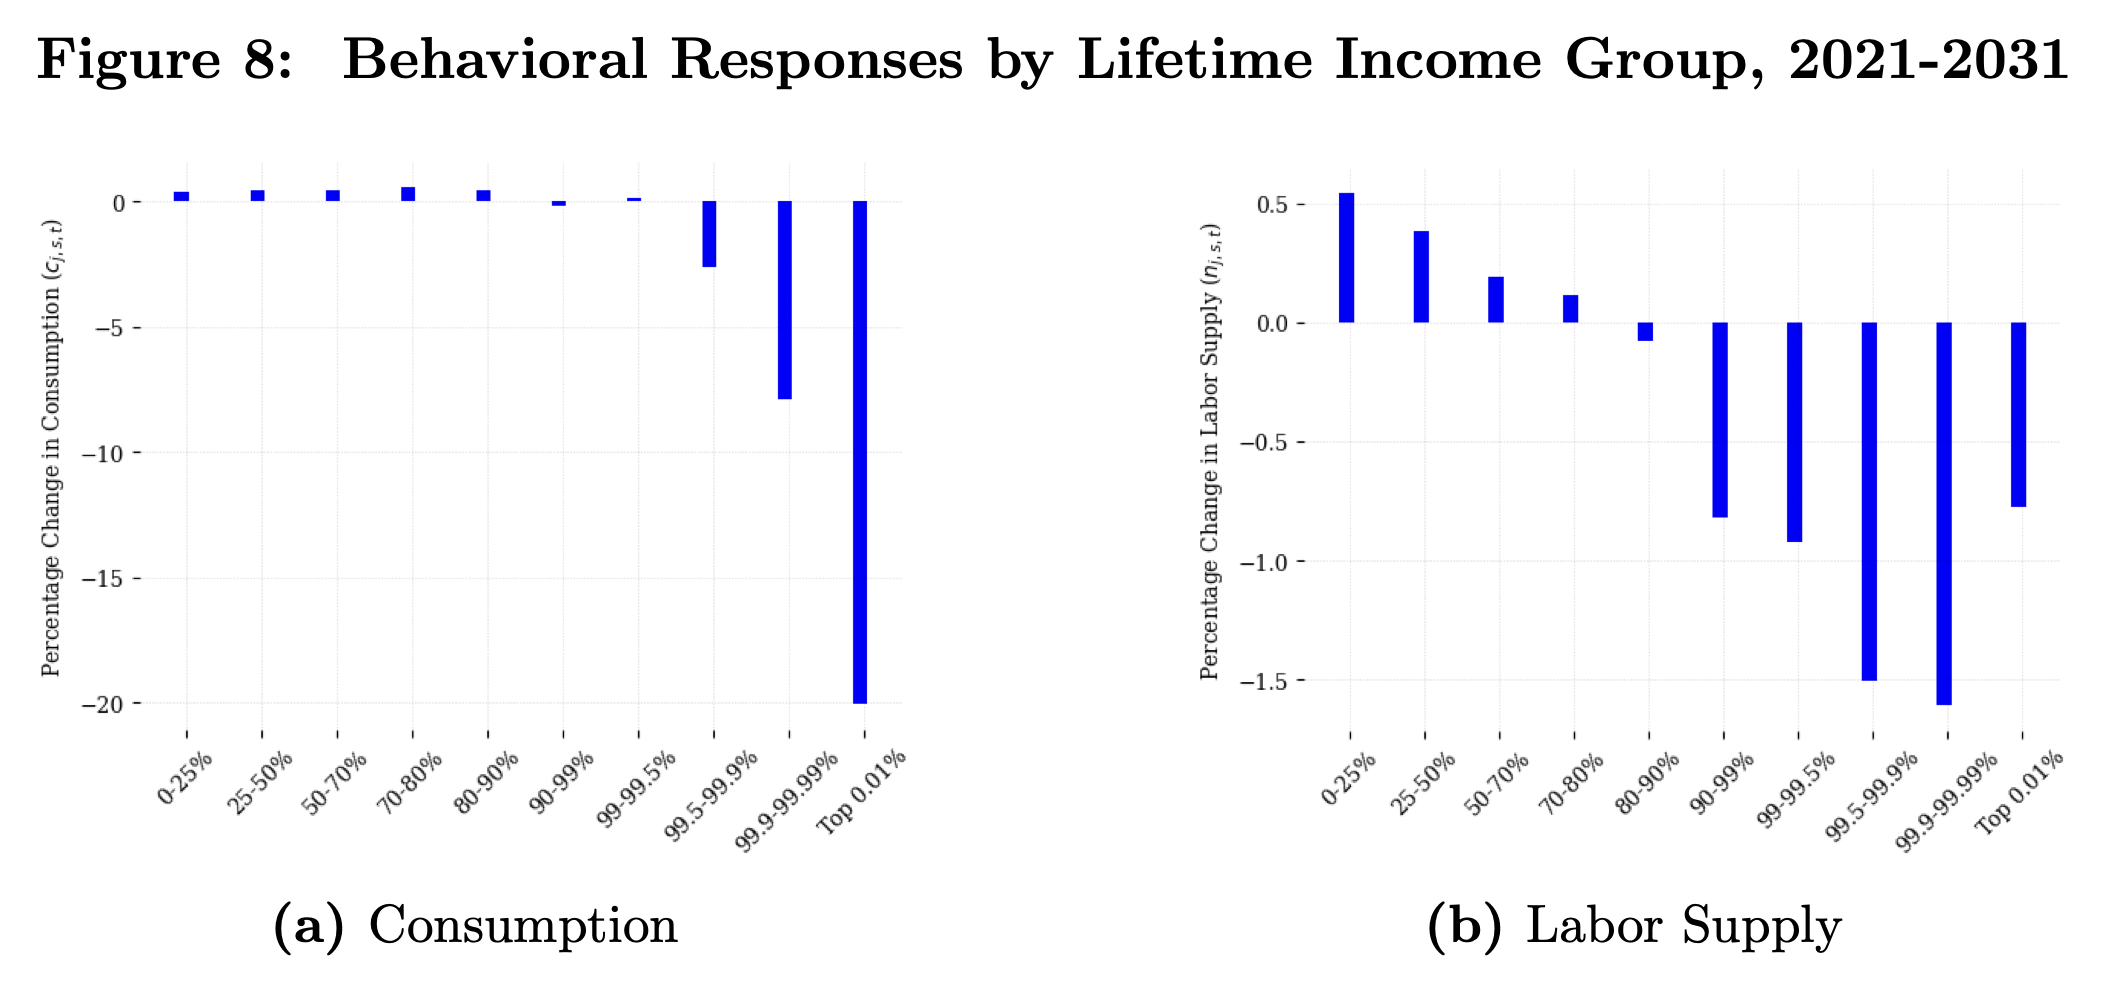
\includegraphics[scale=0.27]{./images/BidenFig8.png}
    \end{figure}
  \end{frame}

  \begin{frame}
  \frametitle{Biden Dynamic Analysis}
    \begin{figure}[htb]\centering
    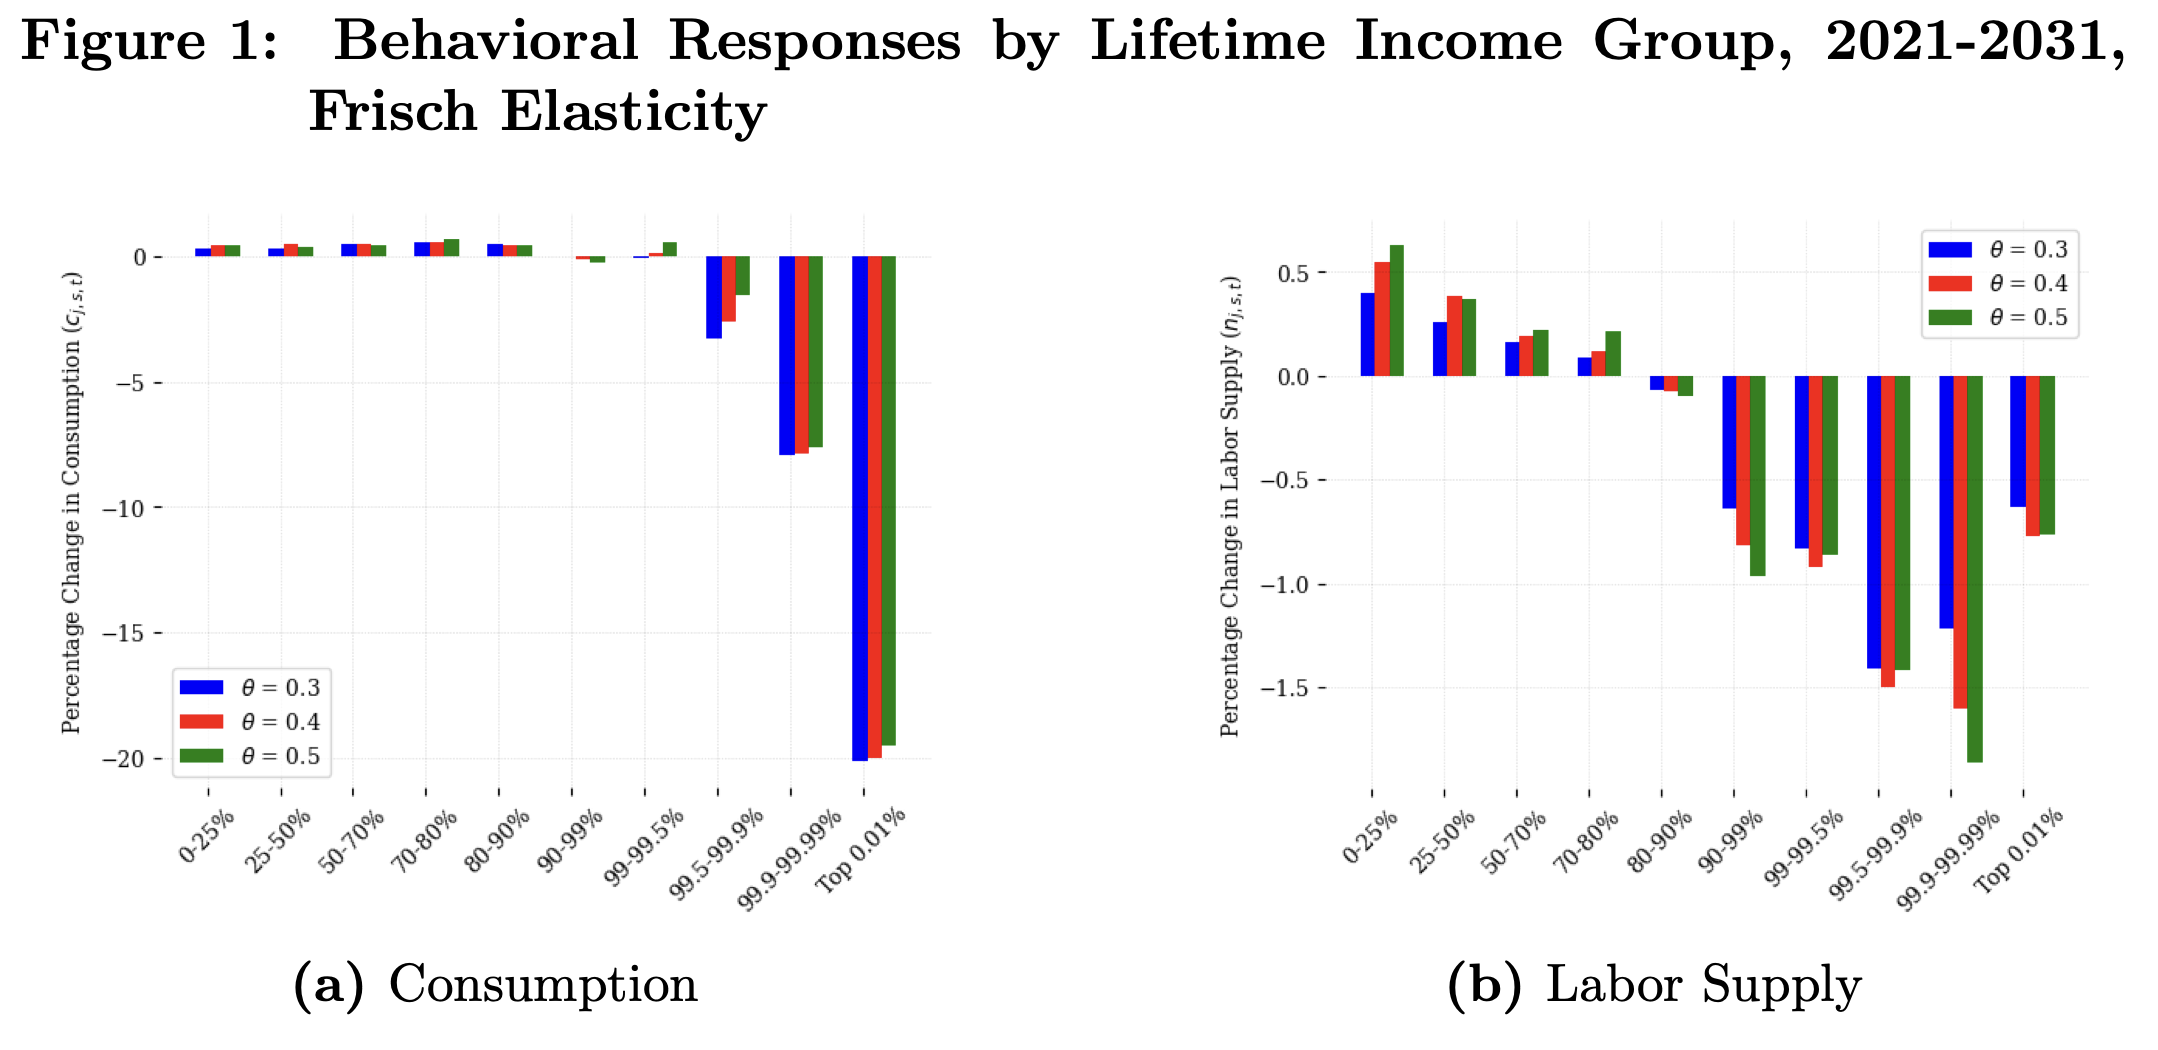
\includegraphics[scale=0.27]{./images/BidenFig1.png}
    \end{figure}
  \end{frame}

\section{Biological Aging}

  \begin{frame}
  \frametitle{The Macroeconomics of Improving Biological Aging}
    \begin{block}{}
      DeBacker, Jason, Richard Evans, and Raiany Romanni, ``The Macroeconomics of Improving Biological Aging'', \textit{Working Paper}, July, 2024.
    \end{block}
    \begin{itemize}
      \item Improving health outcomes leads to large macroeconomic benefits
      \item The time horizons over which health impacts affect the economy can be many decades
    \end{itemize}
  \end{frame}

  \begin{frame}
  \frametitle{Changing Mortality}
    \begin{figure}[htb]\centering
    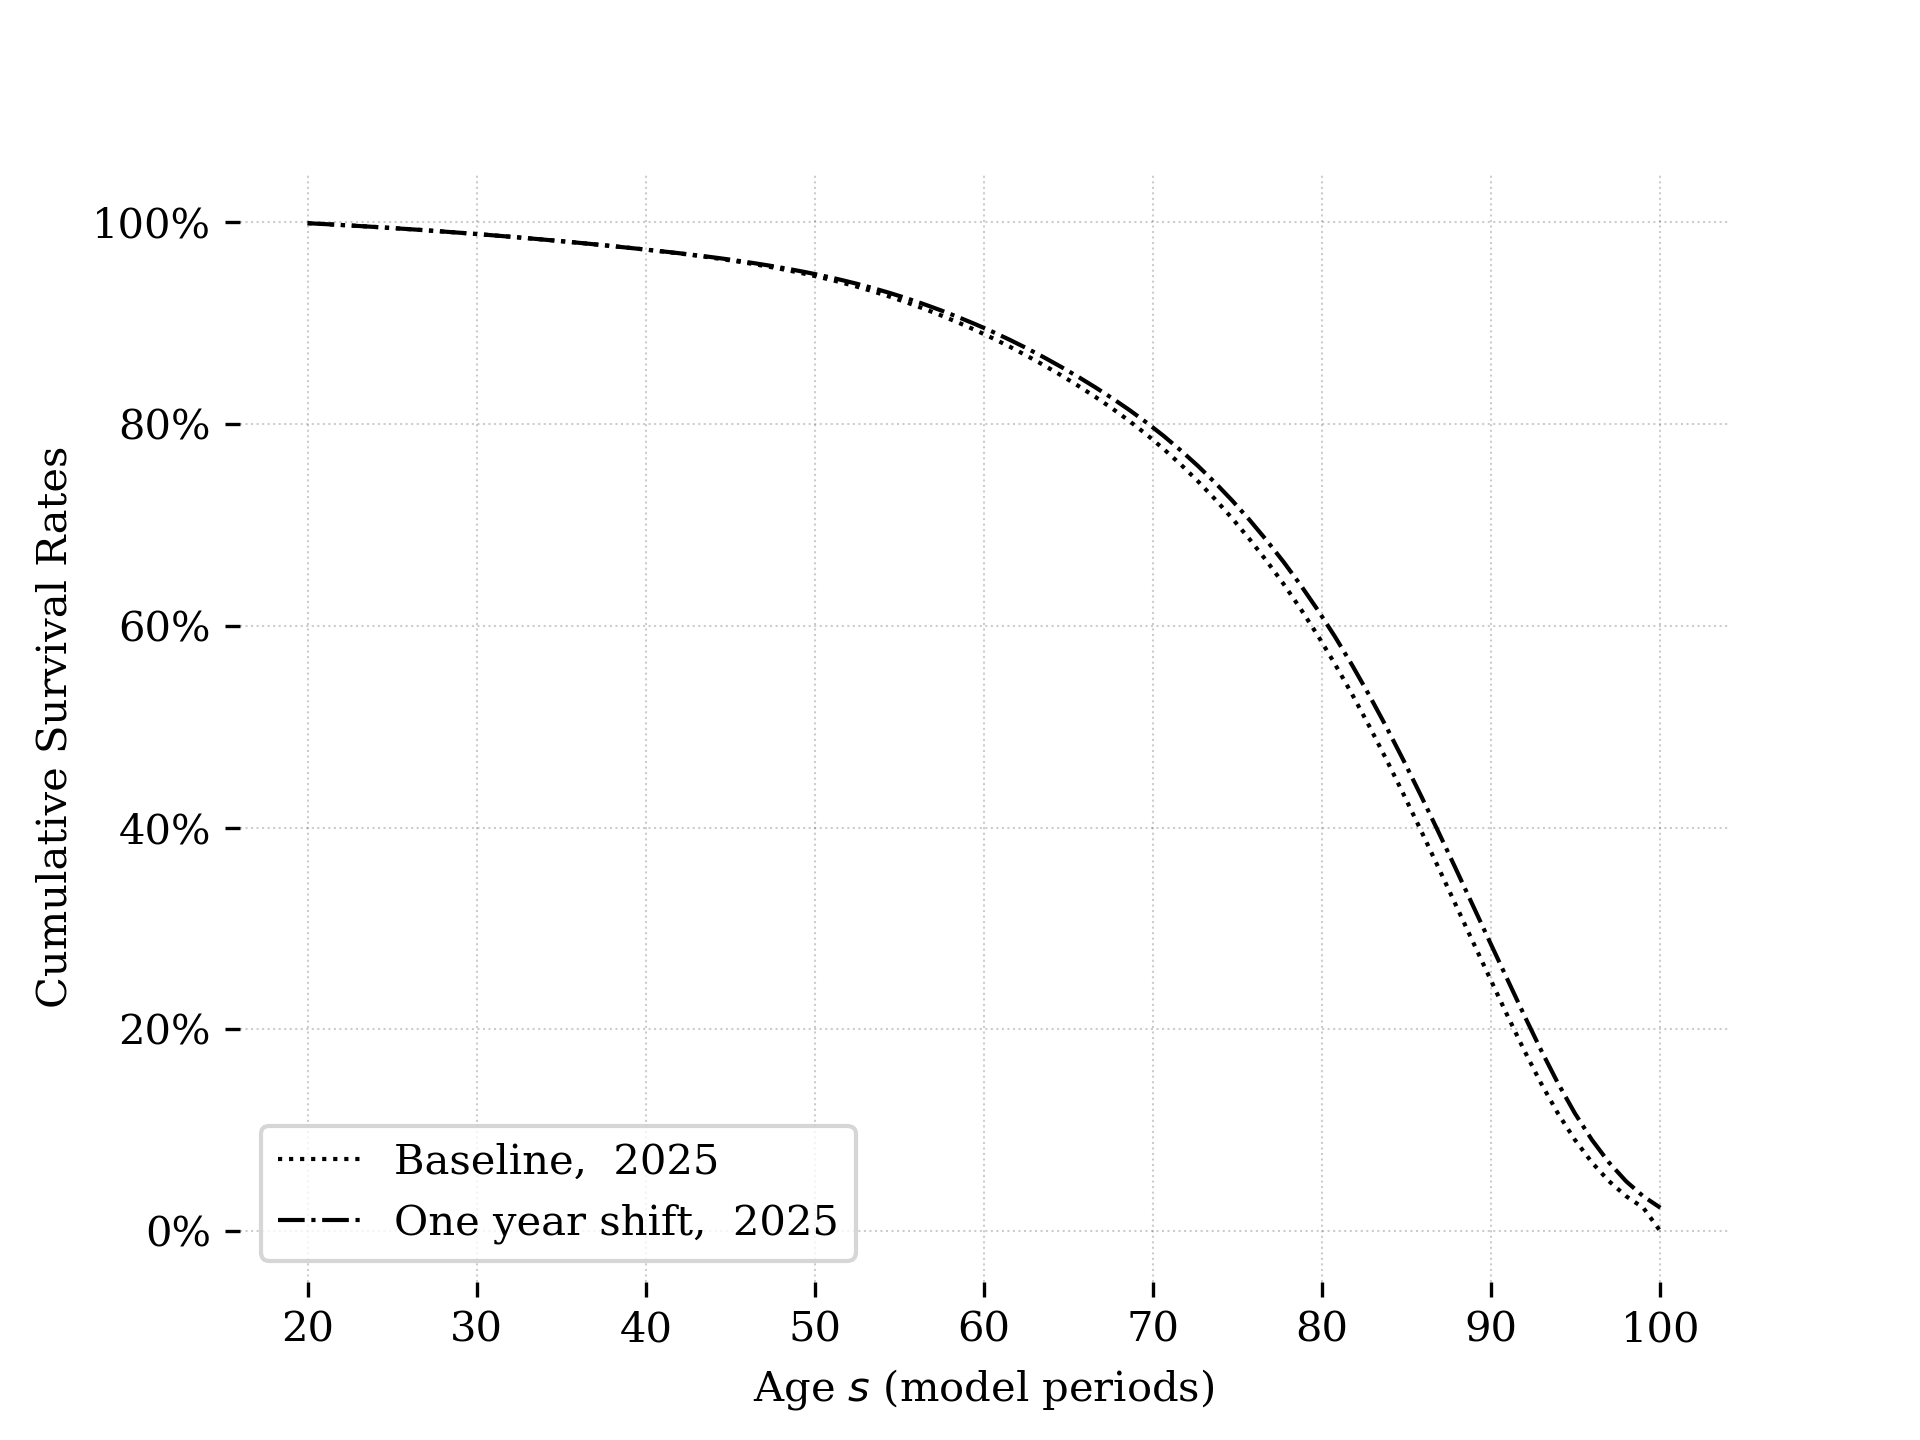
\includegraphics[scale=0.6]{./images/survival_rates.png}
    \end{figure}
  \end{frame}

  \begin{frame}
  \frametitle{Employment Effects}
    \begin{figure}[htb]\centering
      \caption{Employment Paths, One Year Shift in Biological Age}
    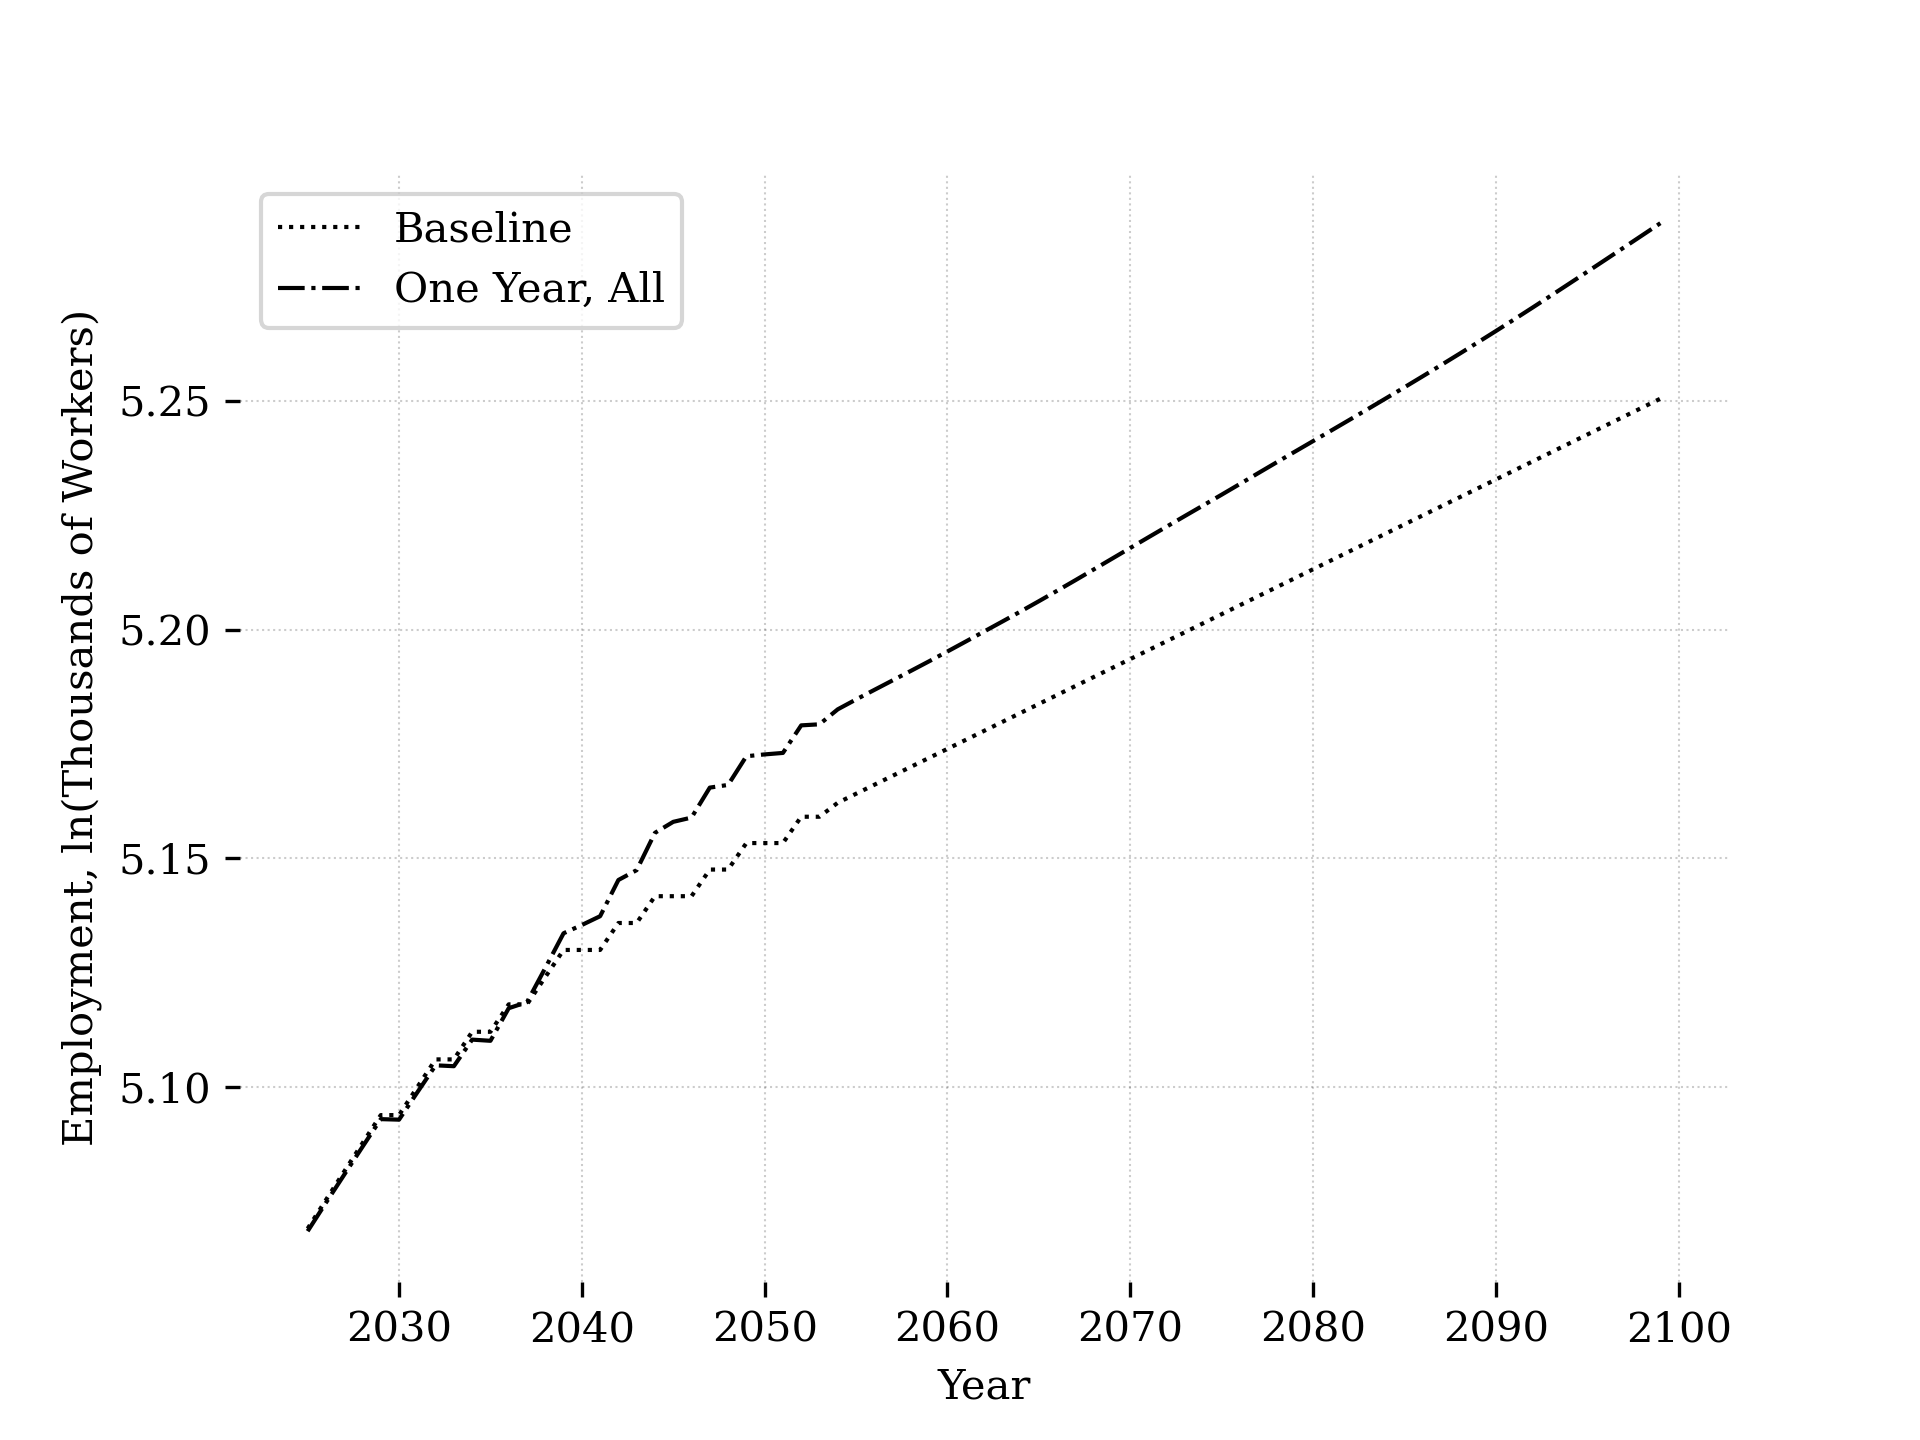
\includegraphics[scale=0.54]{./images/1yrAll_employment_paths.png}
    \end{figure}
  \end{frame}

  \begin{frame}{GDP Effects}
  \begin{table}[h]
    \centering
    \caption{NPV of Change in GDP in Trillions of Constant 2025\$, One Year Shift in Biological Age}
    \label{tab:npv_gdp_1yr}
    % \input{FiguresTables/1yr_npv_gdp_table}
    \begin{tabular}{lrrrr}
    \hline
      Discount Rate & Mortality & Productivity & Fertility & All \\
    \hline
      2\% & 98.52 & 35.75 & 73.21 & 209.86 \\
      4\% & 26.47 & 10.32 & 13.79 & 51.20 \\
      6\% & 8.63 & 3.69 & 2.77 & 15.29 \\
      Model $r$ & 10.40 & 4.47 & 3.25 & 18.06 \\
    \hline
    \end{tabular}
    \end{table}
  \end{frame}


\end{document}
